%%%%%%%%%%%%%%%%%%%%%%%%%%%%%%%%%%%%%%%%%
% Beamer Presentation
% LaTeX Template
% Version 1.0 (10/11/12)
%
% This template has been downloaded from:
% http://www.LaTeXTemplates.com
%
% License:
% CC BY-NC-SA 3.0 (http://creativecommons.org/licenses/by-nc-sa/3.0/)
%
%%%%%%%%%%%%%%%%%%%%%%%%%%%%%%%%%%%%%%%%%

%----------------------------------------------------------------------------------------
%    PACKAGES AND THEMES
%----------------------------------------------------------------------------------------

\documentclass{beamer}

\mode<presentation> {
	
	% The Beamer class comes with a number of default slide themes
	% which change the colors and layouts of slides. Below this is a list
	% of all the themes, uncomment each in turn to see what they look like.
	
	%\usetheme{default}
	%\usetheme{AnnArbor}
	%\usetheme{Antibes}
	%\usetheme{Bergen}
	%\usetheme{Berkeley}
	%\usetheme{Berlin}
	%\usetheme{Boadilla}
	%\usetheme{CambridgeUS}
	%\usetheme{Copenhagen}
	%\usetheme{Darmstadt}
	%\usetheme{Dresden}
	%\usetheme{Frankfurt}
	%\usetheme{Goettingen}
	%\usetheme{Hannover}
	%\usetheme{Ilmenau}
	%\usetheme{JuanLesPins}
	%\usetheme{Luebeck}
	\usetheme{Madrid}
	% \usepackage{listings}
	%\usetheme{Malmoe}
	%\usetheme{Marburg}
	%\usetheme{Montpellier}
	%\usetheme{PaloAlto}
	%\usetheme{Pittsburgh}
	%\usetheme{Rochester}
	%\usetheme{Singapore}
	%\usetheme{Szeged}
%	\usetheme{Warsaw}
	
	% As well as themes, the Beamer class has a number of color themes
	% for any slide theme. Uncomment each of these in turn to see how it
	% changes the colors of your current slide theme.
	
%	\usecolortheme{albatross}
%	\usecolortheme{beaver}
%	\usecolortheme{beetle}
%	\usecolortheme{crane}
%	\usecolortheme{dolphin}
%	\usecolortheme{dove}
%	\usecolortheme{fly}
%	\usecolortheme{lily}
%	\usecolortheme{orchid}
%	\usecolortheme{rose}
%	\usecolortheme{seagull}
%	\usecolortheme{seahorse}
%	\usecolortheme{whale}
%	\usecolortheme{wolverine}
	
%	\setbeamertemplate{footline} % To remove the footer line in all slides uncomment this line
	%\setbeamertemplate{footline}[page number] % To replace the footer line in all slides with a simple slide count uncomment this line
	
%	\setbeamertemplate{navigation symbols}{} % To remove the navigation symbols from the bottom of all slides uncomment this line
%	\usefonttheme{serif}
}
\usepackage{graphicx,wrapfig,lipsum}
\usepackage{graphicx} % Allows including images
\usepackage{booktabs} % Allows the use of \toprule, \midrule and \bottomrule in tables
\usepackage{wrapfig}

\usepackage{subcaption}
\usepackage{tikz}
\usetikzlibrary{decorations.pathmorphing,matrix,decorations.pathreplacing,arrows,decorations.markings}
\usetikzlibrary{fit,calc,shapes,arrows,positioning,shadings,backgrounds,patterns,tikzmark,matrix,spy}
\usetikzlibrary{decorations.markings}

\tikzset{myrow/.style args = {(#1,#2)}{%
		row #1/.style={nodes={fill=#2}}}}

\tikzset{mycolumn/.style args = {(#1,#2)}{%
		column #1/.style={nodes={fill=#2}}}}

\tikzset{mycell/.style args = {(#1,#2,#3)}{%
		row #1 column #2/.style={nodes={fill=#3}}}}

\makeatletter
\usetikzlibrary{chains,patterns,shadows}
\tikzset{% customization of pattern
	% based on <m.wibrow@gm...> - 2013-03-24 07:20: 
	hatch distance/.store in=\hatchdistance,
	hatch distance=5pt,
	hatch thickness/.store in=\hatchthickness,
	hatch thickness=5pt
}
\pgfdeclarepatternformonly[\hatchdistance,\hatchthickness]{north east hatch}% name
{\pgfqpoint{0pt}{0pt}}% below left
{\pgfqpoint{\hatchdistance}{\hatchdistance}}% above right
{\pgfpoint{\hatchdistance-1pt}{\hatchdistance-1pt}}%
{
	\pgfsetcolor{\tikz@pattern@color}
	\pgfsetlinewidth{\hatchthickness}
	\pgfpathmoveto{\pgfqpoint{0pt}{0pt}}
	\pgfpathlineto{\pgfqpoint{\hatchdistance}{\hatchdistance}}
	\pgfusepath{stroke}
}

\newcommand{\KECCAK}{\mbox{\textsc{Keccak}}}
\newcommand{\Keccak}{\mbox{\textsc{Keccak}}}
\newcommand{\SHA}{\textsc{Sha}}
\newcommand{\Rnd}{\textsc{Round}}
\newcommand{\etal}{\textit{et al. }}
%----------------------------------------------------------------------------------------
%    TITLE PAGE
%----------------------------------------------------------------------------------------

\title[Cryptanalysis of Round Reduced \KECCAK{}]{Cryptanalysis of Round Reduced \KECCAK{}} % The short title appears at the bottom of every slide, the full title is only on the title page

\author{Nikhil Mittal} % Your name
\institute[17111056] % Your institution as it will appear on the bottom of every slide, may be shorthand to save space
{
	Under supervision of \\
	\large Prof. Manindra Agrawal and Dr. Shashank Singh\\
	\medskip
	IIT Kanpur \\ % Your institution for the title page
	\medskip
	\textit{nickedes@cse.iitk.ac.in} % Your email address
}
\date{\today} % Date, can be changed to a custom date
% \documentclass[border=10pt]{standalone}

\begin{document}
	\setbeamertemplate{caption}{\raggedright\insertcaption\par}
	
	\begin{frame}
	\titlepage % Print the title page as the first slide
\end{frame}

%\begin{frame}
%\frametitle{Table of Contents}
%\tableofcontents
%\end{frame}

\section{Introduction}

\begin{frame}
	\frametitle{Hash Function}
	\begin{itemize}
		\item $H:\{0,1\}^* \rightarrow \{0,1\}^n $
		\item Deterministic	function
		\item Takes as input a arbitrary size string and outputs a fixed size ($n$) string
		\item Cryptographic applications require it to satisfy the following conditions
		\begin{itemize}\setlength\itemindent{10pt}
			\item {\bf Efficiency}: Given $m$, it is easy to compute $H(m)$.
			\item {\bf Preimage Resistance}: Given $H(m)$, it is computationally hard to find $m$.
			\item {\bf Second-preimage Resistance}: Given $m$, it is computationally hard to find $m^\prime$ such that $H(m)=H(m^\prime)$.
			\item {\bf Collision Resistance}: It is computationally hard to find $m$ and $m^\prime$ such that $H(m)=H(m^\prime)$.
		\end{itemize}
		\item Hash functions having the above properties are referred to as cryptographic hash functions
		\item Used in cryptographic applications such as Authentication, Digital Signatures and Integrity etc..
	\end{itemize}
\end{frame}

\begin{frame}
	\frametitle{Need For \SHA-$3$}
	\begin{itemize}
		\item MD$5$, \SHA-$1$, \SHA-$2$ are very popular hash functions and are widely used
		\item In the year $2005$, the first practical collision attack on MD$5$ was published by Xiaoyun Wang \etal
		\item in the same year, a practical collision attack on \SHA-$0$ and \SHA-$1$ was published by Xiaoyun Wang \etal
		\item NIST was worried about the security of hash functions, though by that time NIST had started using the \SHA-$2$ family of hash functions.
		\item But as \SHA-$2$ was also based on Merkle-Damgard construction like \SHA-$0$, \SHA-$1$, so there was a possibility that it could also be attacked in a similar fashion.
		\item With this thought, in the year $2006$ NIST decided to hold a competition for the next secure hash function.
		\item In $2008$, NIST announced a competition for the Secure Hash Algorithm-$3$ (\SHA-$3$)
		\item 
	\end{itemize}
\end{frame}

\begin{frame}
	\frametitle{\KECCAK{}}
	\begin{itemize}
		\item \KECCAK{} hash function is based on sponge construction
		\item \SHA-$3$ family of hash functions is based on \Keccak{}
		\item The \SHA-$3$ family provides four hash functions: \SHA3-$224$, \SHA3-$256$, \SHA3-$384$ and \SHA3-$512$
		\item Designed to provide resistance against preimage attacks, collision attacks, and second-preimage attacks
		\item  In the year $2012$, NIST announced \KECCAK{} as the winner of the competition among the five finalists viz. BLAKE, Gr\o stl, JH, \KECCAK{} and Skein
		\item Since $2015$, \KECCAK{} has been standardized as \SHA-$3$ by NIST
		\item \Keccak{}'s excellent resistance towards crypt-analytic attacks is one of the main reasons for its selection by NIST. The algorithm is a good mixture of linear as well as non-linear operations.
	\end{itemize}
\end{frame}

\begin{frame}
	\frametitle{Sponge Construction}
	\begin{itemize}
		\item A sponge construction consists of
			\begin{itemize}
				\item A permutation function $f$
				\item a parameter ``rate'' $r$
				\item a padding rule pad
				\begin{figure}
					\resizebox{\linewidth}{!}{
						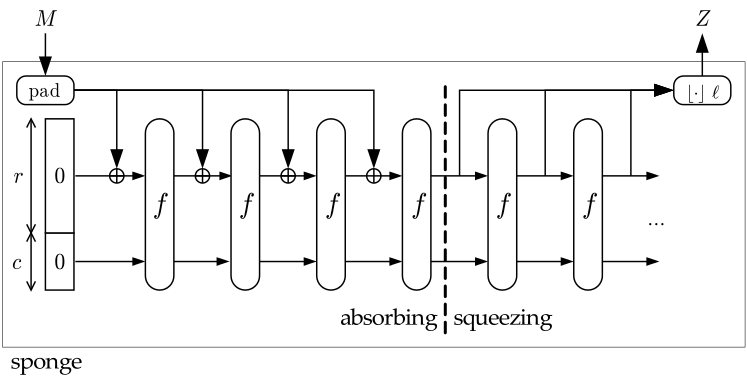
\includegraphics[scale=0.5]{sponge.png}
					}
					\caption{The sponge construction\label{sponge}}
				\end{figure}
				\item This construction produces a sponge function that takes as input a bit string $M$ and generates a string of length $l$
			\end{itemize}
	\end{itemize}
\end{frame}

\begin{frame}
	\begin{itemize}
		\frametitle{\KECCAK{}-$p$ Permutation}
		\item The function $f$ in the sponge construction is denoted by \KECCAK-$f[b]$
		\item $b$ is the length of input string
		\item Internally, \KECCAK-$f[b]$ consists of a round function $p$ which is applied $n_r$ number of times
		\item \KECCAK-$f[b]$ function is specialization of \KECCAK-$p[b, n_r]$
		
	\end{itemize}
\end{frame}
		
\begin{frame}
	\frametitle{State}
	\begin{itemize}
		\item The state input to \KECCAK-$f[b]$ consists of $b$ bits, the state is divided into slices
		\item Size of a slice is fixed i.e., $25$ bits
		\begin{figure}
			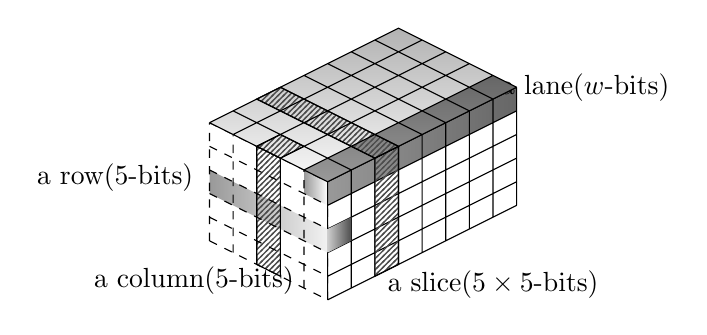
\begin{tikzpicture}[on grid,scale=0.3]
				\shade[yslant=-0.5,right color=gray!10, left color=black!40] (0,2) rectangle +(5,1) node[xshift=-1.2cm, yshift=0.2cm] at (0,2){ a row($5$-bits)};
				%lane 1x1
				\shade[yslant=-0.5,left color=black!40,  color=black!10] (4,4) rectangle +(1,1);
				%column
				\draw[yslant=-0.5,pattern=north east hatch,  pattern color=black!70, hatch distance=3pt, hatch thickness=0.5pt] (2,0) rectangle +(1,5)
				node[xshift=-0.8cm, yshift=-0.2cm] at (2,0){ a column($5$-bits)};
				
				\draw[yslant=-0.5, dashed] (0,0) grid (5,5);
				\shade[yslant=0.5,right color=black!60,left color=black!40](5,-1) rectangle +(8,1);
				\draw[yslant=0.5] (5,-5) grid (13,0);
				\node at (15.9,6.5){a lane($w$-bits)};
				%slice front
				\draw[yslant=0.5,pattern=north east hatch,  pattern color=black!70, hatch distance=3pt, hatch thickness=0.5pt](7,-5) rectangle +(1,5)
				node[xshift=1.5cm, yshift=-0.1cm] at (7,-5){ a slice($5\times 5$-bits)};
				%row front
				\shade[yslant=0.5,left color=black!20,right color=black!70] (5,-3) rectangle +(1,1);
				%top shade
				\shade[yslant=0.5,xslant=-1,bottom color=gray!5,top color=gray!60] (5,0) rectangle +(8,5);
				\shade[yslant=0.5,xslant=-1, bottom color=black!40,top color=black!60](5,0) 
				rectangle +(8,1); 
				%slice top 
				\draw[yslant=0.5,xslant=-1,pattern=north east hatch,  pattern color=black, hatch distance=3pt, hatch thickness=0.5pt] (7,0) rectangle +(1,5);
				%column top
				\draw[yslant=0.5,xslant=-1,pattern=north east hatch,  pattern color=black, hatch distance=3pt, hatch thickness=0.5pt] (5,2) rectangle +(1,1);
				
				\draw[yslant=0.5,xslant=-1] (5,0) grid (13,5);
				\end{tikzpicture}
			\caption{The \KECCAK{} State \label{ss}}
		\end{figure}
	\end{itemize}
\end{frame}

To see how the \texttt{chemfig} package creates the drawings from your code, let us look at the simple water molecule:

\vskip 0.3cm
\begin{center} 
\chemfig{H_2O} is created with \verb|\chemfig{H_2O}|
\end{center}

The simple \LaTeX{} code on the right is automatically converted into the molecular formula for water on the left. 
\vskip 0.3cm
Rings are similarly easy to code - consider the examples below:

\vskip 0.3cm

\chemfig[][scale=0.5]{A*5(-B-C-D-E-)} = \verb|\chemfig{A*5(-B-C-D-E-)}|

\vskip 0.3cm

\chemfig[][scale=0.5]{*6(=-=-=-)} = \verb|\chemfig{*6(=-=-=-)}|


\end{frame}

\section{Where to go next\dots{}}

\begin{frame}{Where to go next\dots{}}

\begin{itemize}
\item This short example was designed to introduce you to using Overleaf for scientific presentations.
\item This is made possible by the many great packages that have been developed for \LaTeX{}, including the two we focused on here (plus the \texttt{Beamer} package used for the overall presentation style). 
\item For more help on using \LaTeX{}, see the links on the Overleaf help page: \url{www.overleaf.com/help} or check out our free introductory course: \url{www.overleaf.com/blog/7}.
\end{itemize}

\begin{center}
Follow @overleaf on Twitter for all the latest news and updates.\\[0.3cm]
Happy \LaTeX ing!
\end{center}

\end{frame}

\end{document}